\documentclass[11pt,a4paper]{article}
\usepackage[utf8]{inputenc}
\usepackage[margin=1.15in]{geometry}
\usepackage{amsmath,amssymb}
\usepackage{booktabs,longtable,array}
\usepackage{graphicx}
\usepackage{pdflscape}
\usepackage{placeins}
\usepackage{threeparttable}
\usepackage[authoryear,round]{natbib}
\usepackage[font=small,labelfont=bf]{caption}
\usepackage{xcolor}
\usepackage[colorlinks=true,linkcolor=blue!50!black,citecolor=blue!50!black,urlcolor=blue!50!black]{hyperref}
\linespread{1.12}
\setlength{\parskip}{0.4em}
\setlength{\parindent}{1.2em}

\title{\textbf{Offsetting by Mandate, Not by Choice:}\\[2pt] Tax-Point Swaps and Vertical Fiscal Interaction\\ among Swiss Municipalities}
\author{Eduardo Dietrich Zimmermann}
\date{September 2026\\[2pt] \small Working paper draft --- writing sample for the PhD application at the KOF Swiss Economic Institute, ETH Zurich}

\begin{document}
\maketitle

\begin{abstract}\noindent
In Switzerland, cantons and municipalities tax the same income by levying multipliers on a common ``simple tax'', so that one point of the cantonal multiplier and one point of the municipal multiplier are perfect substitutes from the taxpayer's perspective. I ask whether municipalities offset changes in the cantonal multiplier, and whether offsets arise by law or by choice. I combine multipliers for 1,916 municipalities with stable boundaries (2010--2025), the historised municipality register and municipal boundaries, and document 45 cantonal changes of at least two points. Six are compensatory \emph{swaps}, in which canton and municipalities move in opposite directions by almost the same amount; in the four large ones the median municipal offset is 0.97, and in Neuch\^atel and Vaud the reallocation persists for at least four years with the combined burden unchanged. For the remaining 39 changes, the voluntary municipal offset is indistinguishable from zero (cumulative offset $-0.01$, 95\% CI $[-0.07,\,0.06]$) and pass-through to the combined burden is 0.99. Municipalities adjacent to another canton do not respond to that canton's multiplier changes, nor (with much lower precision) to its pure swaps. A descriptive case study of Luzern's 2020 reform (AFR18) shows the observed revenue loss from the swap was more than compensated by transfers, and that most municipalities kept the mandated multiplier when the mandate ceased to bind, irrespective of their projected fiscal burden from the reform. Checks with effective tax burdens for a single taxpayer give consistent but less precise results. Leading co-movement in the data cautions against a causal reading of dynamics beyond the swaps themselves.
\medskip

\noindent\textbf{JEL:} H71, H73, H77 \quad \textbf{Keywords:} fiscal federalism, vertical tax externalities, tax multipliers, Switzerland, municipalities
\end{abstract}

\section{Introduction}

Swiss cantons and municipalities tax the same income. Both levy their income taxes as multiples (\emph{Steuerf\"usse}) of a common ``simple tax'' computed under cantonal law, so a household's combined cantonal--municipal burden is proportional to the sum of the two multipliers. A point of cantonal multiplier and a point of municipal multiplier are therefore perfect substitutes for the taxpayer, but not for the governments that collect them. This makes the Swiss multiplier system an unusually clean setting for two questions at the centre of fiscal federalism. First, when a canton changes its multiplier, do municipalities respond in the offsetting direction, internalising the vertical externality that each tier exerts on the other's tax base \citep[as in][]{KeenKotsogiannis2002}? Second, when offsetting does occur, does it come from municipal choice or from legislation?

I argue that, in the data, offsets are legislated rather than chosen. Cantons occasionally execute a \emph{tax-point swap}: the canton raises (or lowers) its multiplier by $x$ points and its municipalities simultaneously lower (raise) theirs by the same $x$; in Luzern this was legally mandated as part of the counter-financing of a reallocation of tasks. I assemble a panel of 1,916 municipalities with stable boundaries for 2010--2025 from the multipliers published by the Swiss Federal Tax Administration (ESTV), the historised municipality register of the Federal Statistical Office and the municipal boundaries of swisstopo, and identify 45 canton-level multiplier changes of at least two points. Six of them are swaps, recognisable by a near-uniform, simultaneous, opposite-signed move of virtually all municipalities. In the four large swaps (Luzern 2020, Neuch\^atel 2014, Vaud 2011 and 2012) the median same-year municipal offset is 0.97 points per point of cantonal change. Relative to clean control cantons, the combined burden hardly moves, and in Neuch\^atel and Vaud the new split between tiers is still in place four to five years later.

For the other 39 changes there is no such mandate, and there is no sign of voluntary offsetting. In a distributed-lag model of municipal multiplier changes on cantonal changes, with year fixed effects and cantonal leads, the cumulative offset over four years is $-0.008$ (standard error 0.033); its 95\% confidence interval rules out offsets larger than about seven percent of the cantonal change. Pass-through of unilateral cantonal changes to the combined burden is 0.99. Horizontal responses are equally absent: municipalities adjacent to another canton, compared with interior municipalities of the same canton and year, do not react to that neighbour's multiplier changes (cumulative response $-0.05$, s.e.\ 0.04), nor to the mandated municipal-rate changes generated by its swaps (imprecise, $-0.01$, s.e.\ 0.17). The latter is a test of whether local politicians mimic a neighbour's \emph{headline} municipal rate even when the neighbour's residents face no change in their combined burden.

The paper's third element is a case study of the largest swap, Luzern's 2020 tax reform (AFR18). Revenue from direct taxes on natural persons in 21 larger Luzern municipalities falls by about five to seven percent relative to control cantons, in line with the ten-point cut in multipliers, while transfer revenue rises by 14--28 percent and operating expenditure by 5--9 percent, so the swap was accompanied by a large expansion of gross flows and roughly neutral net balances. The Federal Supreme Court ruled in May 2020 that the mandated municipal reduction violated municipal autonomy; nevertheless, only one of 71 stable Luzern municipalities deviated from the mandated multiplier in 2020, and in 2021, when they were free to choose, three quarters left their multiplier unchanged while 15 percent reversed the swap in full; reversals are unrelated to each municipality's projected fiscal burden from the reform. The swap outlived the mandate.

\paragraph{Caveats.} The evidence rests on institutional variation and design-based comparisons rather than on experimental assignment. The number of mandated swaps is small (four events in three cantons), so estimates specific to swaps are descriptive; for the voluntary-response estimates, municipal multipliers tend to co-move with cantonal multipliers two years \emph{before} a cantonal change, which I report and which limits a causal reading of the dynamics. Multipliers are statutory rates, not effective tax burdens; a check with effective burdens for one household type (Section~\ref{sec:burden}) gives consistent but less precise results.

\paragraph{Contributions.} The paper (i) documents 45 cantonal multiplier changes in 2011--2025 and classifies six of them as swaps; (ii) shows that, outside these episodes, municipalities exhibit no detectable voluntary offset (an informative estimate that excludes offsets larger than about seven percent, subject to the caveat on leads); (iii) shows that the reallocation persists for several years in Neuch\^atel and Vaud; (iv) finds no precisely estimated cross-border response to neighbouring cantons' changes, while the pure-swap estimate is too imprecise to settle headline-rate mimicry; and (v) provides a descriptive case study of Luzern's AFR18, showing the mechanics of a mandated swap and the persistence of the municipal default after the mandate was struck down, with inconclusive evidence on fiscal absorption.

\paragraph{Related literature.} The theoretical starting point is \citet{KeenKotsogiannis2002}: when tiers of government tax the same base, each ignores the effect of its own rate on the other's revenue, which creates a vertical fiscal externality that, under plausible conditions on how governments order immobile and mobile tax bases, biases combined taxation upward relative to the horizontal-competition benchmark of excessive undertaxation. \citet{BruelhartJametti2006} test vertical against horizontal externalities directly in a panel of Swiss municipalities and find that the vertical channel dominates, so that cantonal and municipal rates on the same base move together rather than apart; \citet{FeldKirchgaessner2001} document income-tax competition between cantons and, separately, between municipalities within cantons. My results add a complementary fact to this literature: the co-movement these papers detect need not reflect active vertical coordination by municipalities, since I find no evidence of a voluntary response once mandated swaps are set aside. \citet{Parchet2019} instruments each municipality's neighbours' tax rate with the rate of the neighbouring canton for municipalities located near a cantonal border and finds that municipal rates are strategic substitutes. My cross-border design exploits the same source of variation, the neighbouring canton's rate, but works in first differences with canton-by-year fixed effects, and separates neighbouring cantons' ordinary rate changes from their pure swaps, which alter the neighbour's municipal rate without altering its own residents' combined burden. Broader surveys of the empirical literature on strategic interaction among governments are in \citet{Brueckner2003}; \citet{Agrawal2015} identifies local tax setting from discontinuities at jurisdictional borders, and \citet{Isen2014} uses close local referenda in Ohio to test for fiscal spillovers between overlapping and neighbouring local governments, finding none. \citet{BesleyCase1995} link local rate setting to yardstick competition among incumbents, one candidate mechanism, alongside simple imitation, for the headline-rate mimicry that my cross-border test is designed to detect.

The remainder of the paper is organised as follows. Section~\ref{sec:inst} describes the institutions. Section~\ref{sec:data} describes the data and the classification of events. Section~\ref{sec:strategy} presents the empirical strategy. Section~\ref{sec:results} reports results, and Section~\ref{sec:disc} discusses limitations. Section~\ref{sec:concl} concludes.

\section{Institutional background}\label{sec:inst}

\subsection{The multiplier system}
In most Swiss cantons, cantonal and municipal income taxes are computed as multiples of a simple tax determined by cantonal tax law; the multiplier of the canton is set by the cantonal parliament (and sometimes by referendum), while each municipality sets its own, typically in the annual budget process. The combined burden of a household is proportional to $c+m$, the sum of the cantonal multiplier $c$ and municipal multiplier $m$ (church taxes are set separately and are ignored here). The ESTV publishes both multipliers for every municipality every year. Because $c$ is uniform within a canton, changes in $c$ are shocks common to all municipalities of a canton, while $m$ varies between municipalities.

\subsection{Conceptual framework}\label{sec:concept}
The multiplier system gives the vertical-externality argument of \citet{KeenKotsogiannis2002} an unusually direct empirical counterpart. Because canton and municipality tax the same base, an increase in $c$ raises the effective price of local public funds for every municipality in the canton: on the margin, a franc of municipal spending now competes with a heavier combined tax burden for the same taxpayer. A municipal government that internalises this externality, in the sense of caring about the combined burden $c+m$ faced by its residents, would respond to an increase in $c$ with at least a partial cut in $m$. The degree to which it does so is an empirical question, and it is the one this paper answers directly: the cumulative-offset parameter $\Theta$ defined in Section~\ref{sec:strategy} is $-1$ under full internalisation and $0$ under none. A municipality's multiplier can also move for reasons unrelated to the canton's decision, notably in response to its \emph{horizontal} neighbours: standard tax-competition logic predicts that neighbouring jurisdictions' rates move together if bases are attracted by low taxes (strategic complementarity) or apart if governments free-ride on shared amenities (substitutability), and empirical results for Swiss municipalities have found evidence of the latter \citep{Parchet2019}. Sections~\ref{sec:strategy} and~\ref{sec:results} are designed to keep these two channels apart: the distributed-lag design isolates the vertical response to a municipality's own canton, while the cross-border design isolates the horizontal response to a neighbouring canton, and both are further split into their mandated and voluntary components using the swap classification of Section~\ref{sec:data}. A null result for the voluntary channels is informative in its own right: it says that active vertical or horizontal coordination by municipal governments is not detectable in the multiplier data, not that the underlying externalities are absent, since frictions in local politics, bounded attention, or simply the difficulty of attributing a canton's decision to one's own tax bill could all prevent a response without implying that residents are indifferent to their combined burden.

\subsection{Tax-point swaps}
A canton may transfer a task, or the financing of a task, from municipalities to itself. To keep the reform roughly neutral for the two tiers, it can raise its own multiplier by $x$ points and require municipalities to lower theirs by $x$. For taxpayers, $c+m$ is unchanged. For governments, revenue shifts from municipalities to the canton in proportion to each municipality's tax base, which differs greatly across municipalities. The swap is therefore fiscally neutral for taxpayers and for the two tiers in aggregate, but redistributive across municipalities unless compensated by transfers or equalisation. In Section~\ref{sec:data} I identify swaps from the pattern of municipal multiplier changes; I do not rely on legal documentation except for Luzern.

\subsection{Luzern's AFR18}
The Task and Finance Reform 18 (\emph{Aufgaben- und Finanzreform 18}, AFR18) of the Canton of Luzern was adopted by the cantonal parliament on 18 February 2019 and entered into force on 1 January 2020 \citep{BGer2020}. It rebalanced the financing of tasks between the canton and municipalities (a new cost split for compulsory schooling was a central element of the proposal put to consultation, \citealp{GemeindenLU2018}) and was designed to be roughly cost-neutral for canton and municipalities as a whole; it was counter-financed among other things through a tax-point swap and adjustments to fiscal equalisation \citep{KantonLU2019}. The swap was written into a separate, temporary law: for the fiscal year 2020 it set the cantonal multiplier at 1.70 units, up from 1.60, and the municipal multipliers at their 2019 values minus 0.10 units \citep{BGer2020}. In the City of Luzern, for example, the municipal multiplier fell from 1.85 to 1.75 units \citep{StadtLU2020}. The cantonal ballot brochure states that, in the aggregate balance of the reform, no municipality would be burdened by more than CHF 60 per capita and year \citep{KantonLU2019}.

On 18 May 2020 the Federal Supreme Court held that removing the municipalities' competence to set their own multiplier violated municipal financial autonomy, set the mandated reduction aside, and left the remainder of AFR18 in force \citep{BGer2020}. As reported at the time, municipalities could set a different multiplier for 2020, but where they did not the multiplier fixed by the reform remained in place \citep{SRF2020}; the City of Luzern's executive proposed not to adjust its 2020 multiplier retroactively \citep{StadtLU2020}. This sequence turns the swap, from May 2020 onward, into a \emph{default} rather than a requirement, which I exploit in Section~\ref{sec:lu}.

\section{Data and event classification}\label{sec:data}

\paragraph{Multipliers.} I use the ESTV income-tax multipliers of all cantons and municipalities for 2010--2025 (cantonal $c_{kt}$ and municipal $m_{it}$, in percent of the simple tax). The panel has 2,691 distinct municipality codes across the 16 years, and all 26 cantons appear every year. Within a canton and year, the cantonal multiplier is uniform.

\paragraph{Municipal mergers.} Between 2011 and 2025, waves of mergers, notably in Glarus (2011), Vaud, Ticino, Bern and Graub\"unden, change municipal identity and boundaries. I use the historised municipality register (eCH-0071, status 1 January 2026) to identify every municipality involved in a merger mutation and remove it from the sample: 754 municipality identifiers are involved in mergers effective 2011--2025, 562 of which no longer exist. These identifiers account for 97.5 percent of the 570 codes that disappear from the multiplier panel. The \emph{stable} sample consists of the 1,916 municipalities present in all 16 years and not involved in any merger (Appendix~\ref{app:data}).

\paragraph{Geography.} I use the 2026 boundaries of swissBOUNDARIES3D to construct polygon adjacency. There are 6,073 adjacent municipality pairs, of which 899 span a cantonal border; 656 of the 1,896 municipalities of the estimation sample have at least one neighbour in another canton.

\paragraph{Municipal finances and tax base.} For the case study I use the Federal Finance Administration's municipal financial statistics (accounts by type and function, municipalities with at least 5,000 inhabitants, 2008--2024; account 400 is direct taxes on natural persons, primarily income and wealth taxes) and the ESTV's federal direct tax statistics for individuals by municipality (2010--2019 used), from which I take per-capita federal tax yield as a proxy for fiscal capacity.

\paragraph{Effective tax burdens.} From the tax burden statistics of the ESTV's Swiss Tax Calculator I export, for each year 2010--2025, the burden of a single taxpayer without children and without church membership, with gross labour income of CHF 100,000, in every municipality \citep{ESTV2026}. Each file reports the total burden and its federal, cantonal, communal, church and personal components. In every year the number of rows equals the number of municipalities in the multiplier panel, the components add up to the total exactly, and the municipality codes match the multiplier panel in all cases. Since the communal tax is the municipal multiplier times the same simple tax as the cantonal tax, the communal-to-cantonal burden ratio reproduces the multiplier ratio in about 92 percent of municipality-years; the exceptions are Valais and Geneva in all years, and Vaud in 2024--2025. The calculation rules differ from those of the former annual publication (for example, the direct federal tax is now included), so I use only the calculator series.

\paragraph{Projected fiscal effects of AFR18.} For Luzern I extract the canton's \emph{Globalbilanz 1} (version of the ballot brochure, figures as of the parliamentary committee of 31 January 2019), which reports for each of the 83 municipalities the projected annual effect of every AFR18 measure and of half of the federal-reform (STAF) revenue, in francs and francs per inhabitant, with a negative sign denoting a burden \citep{GlobalbilanzLU2019}. The table is internally consistent: the components add up to the reported totals within CHF 3, and the municipal columns add up to the reported totals for municipalities within CHF 6. The swap column is the revenue effect of ten multiplier points on the 2016 tax base: for the 21 municipalities in the financial statistics, multiplier times base implied by this column reproduces the 2016 revenue from direct taxes on natural and legal persons (accounts 400 and 401) with a median ratio of 1.01 and a log correlation of 1.00. Projected net effects range from a burden of CHF 510 per inhabitant (Meggen) to a relief of CHF 406 (Altwis). This version precedes the hardship compensation described in the ballot brochure, which caps the burden at CHF 60 per inhabitant \citep{KantonLU2019}, and therefore overstates the burden of the worst-affected municipalities.

\paragraph{Canton-level changes.} A cantonal change is a canton-year with $|\Delta c_{kt}|\ge 2$ points. I find 47 such changes between 2011 and 2025. I drop the two Appenzell Ausserrhoden events (2014, 2018), which coincide with implausible municipal jumps in the source data, leaving 45 events in 18 cantons. For each event I compute the same-year change $\Delta m_{it}$ of the stable municipalities in the canton, and the share of municipalities whose move offsets the cantonal change to within one point.

\paragraph{Classification.} An event is a \emph{mandated swap} if at least 10 stable municipalities are observed, at least 80 percent of municipalities offset the cantonal change to within one point and at least 85 percent move in the opposite direction; a \emph{small-canton swap} if fewer than 10 municipalities are observed, all move in the opposite direction and the mean is within two points of an exact offset; all others are \emph{unilateral}. The classification conditions on the same-year municipal response. This is defensible because a near-uniform, simultaneous, opposite-signed move of nearly all municipalities is difficult to reconcile with independent voluntary rate-setting and is therefore classified as a mandated swap; but it means partial responses are kept in the unilateral class, which, if anything, biases the unilateral offset toward finding one (Table~\ref{tab:robust} shows the result without cantons that have partial swaps). For Luzern the legal mandate is documented (Section~\ref{sec:inst}); for the other episodes the classification is empirical, and I do not claim to have audited the legal basis of each reform.

\begin{table}[t]\centering\small
\caption{Canton-level multiplier changes of at least two points, 2011--2025}\label{tab:classes}
\resizebox{\textwidth}{!}{\begin{tabular}{lccccccc}
\toprule
Class & Events & Cantons & Mean $|\Delta c|$ & Median offset & Share opposite & Share unchanged \\
\midrule
Mandated swap & 4 & 3 & 6.5 & 0.97 & 0.96 & 0.03 \\
Small-canton swap & 2 & 2 & 8.0 & 0.89 & 1.00 & 0.00 \\
Unilateral change & 39 & 14 & 7.6 & $-0.06$ & 0.14 & 0.67 \\
\bottomrule
\end{tabular}}

\vspace{2pt}\parbox{\textwidth}{\footnotesize \emph{Notes:} ``Offset'' is $-\overline{\Delta m}/\Delta c$ for the event (1 = full offset). ``Share opposite'': share of stable municipalities moving opposite to the cantonal change in the same year; ``unchanged'': share with $\Delta m=0$. Cantons: mandated swaps in LU (2020), NE (2014), VD (2011, 2012); small-canton swaps in AI (2011), BS (2017). The full list is in Appendix Table~\ref{tab:events}.}
\end{table}

Table~\ref{tab:classes} and Figure~\ref{fig:events} summarise the result. The two groups are strikingly different. Mandated swaps lie on the anti-diagonal of Figure~\ref{fig:events}: 96 percent of municipalities move in the offsetting direction in the same year and only 3 percent leave their multiplier unchanged. For the 39 unilateral changes, two thirds of municipalities do not change their multiplier in the year of the cantonal change, and only 14 percent move in the offsetting direction, which is close to what one would expect from the background rate of municipal changes, since in the overall panel 75 percent of municipality-years show no change in the multiplier.

\begin{figure}[t]\centering
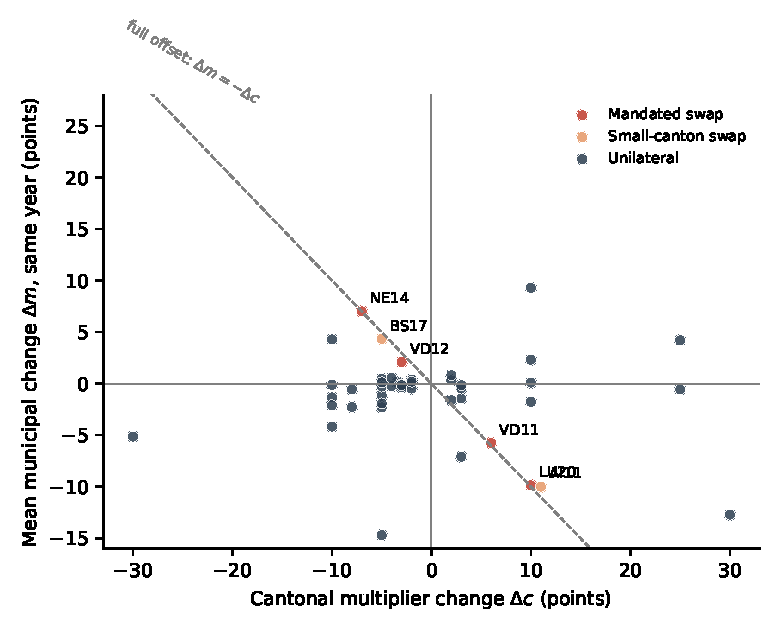
\includegraphics[width=0.62\textwidth]{figs/fig1_events.pdf}
\caption{Cantonal and average municipal multiplier changes in the same year}\label{fig:events}
\parbox{0.9\textwidth}{\footnotesize \emph{Notes:} Each dot is a canton-year with $|\Delta c|\ge2$ points (AR excluded). The dashed line is a full offset, $\Delta m=-\Delta c$.}
\end{figure}

\section{Empirical strategy}\label{sec:strategy}

\subsection{Mandated swaps: event studies against clean controls}
For each of the three swap episodes with sufficient municipalities (LU 2020, NE 2014, VD 2011--12), I compare the change in the average municipal multiplier, and in the combined burden $c+m$, from the year before the swap to each year in a window of four years before and up to five years after, to the corresponding change in control cantons. Control cantons are those with no cantonal change of one point or more in the window. Placebo paths are obtained by treating each control canton in turn as the swapping canton, in the spirit of placebo-in-space inference \citep{Abadie2010,ConleyTaber2011}. With a single treated canton per event, formal $p$-values are not informative; the figures show the distribution of placebo paths. The comparison follows the clean-control logic of stacked event designs \citep{Cengiz2019} and avoids the contamination of two-way fixed-effects estimates by heterogeneous timing \citep{GoodmanBacon2021}.

\subsection{Voluntary responses: distributed lags in first differences}
For municipality $i$ in canton $k$, let $\Delta m_{it}$ be the change in its multiplier, $\Delta c^{U}_{kt}$ the cantonal change in years that are not classified swaps and $\Delta c^{S}_{kt}$ the cantonal change in classified swap years. I estimate
\begin{equation}
\Delta m_{it}=\sum_{\ell=-2}^{3}\beta_\ell\,\Delta c^{U}_{k,t-\ell}+\sum_{\ell=0}^{2}\delta_\ell\,\Delta c^{S}_{k,t-\ell}+\lambda_t+\varepsilon_{it},
\label{eq:dl}
\end{equation}
with year effects $\lambda_t$ and standard errors clustered by canton (24 clusters). The parameter of interest is the cumulative offset $\Theta=\sum_{\ell=0}^{3}\beta_\ell$: $\Theta=-1$ means a full offset and $\Theta=0$ means none, so pass-through to the combined burden is $1+\Theta$. Coefficients on leads ($\ell<0$) test whether municipalities change multipliers ahead of cantonal changes. Because the regressors vary at the canton-year level, I complement clustered inference by a permutation test that randomly reassigns entire canton paths of the unilateral cantonal changes (leads and lags together) across the 24 cantons of the estimation sample, holding the swap variables fixed; it uses 1,000 random permutations and two-sided $p$-values based on the absolute value of the coefficient. The identifying assumption is that, conditional on year effects and leads, cantonal changes are unrelated to contemporaneous municipal-level innovations in the multiplier. It is plausible for the average municipality, since cantonal changes are decided by cantonal parliaments, but not guaranteed, and I test it through the leads and drift controls.

\subsection{Cross-border responses}
For municipality $j$ let $\mathcal N_j$ be the set of adjacent municipalities located in another canton. Define
\[
N^{U}_{jt}=\frac{1}{|\mathcal N_j|}\sum_{i\in\mathcal N_j}\Delta c^{U}_{k(i),t},\qquad N^{S}_{jt}=\frac{1}{|\mathcal N_j|}\sum_{i\in\mathcal N_j}\left(-\Delta c^{S}_{k(i),t}\right),
\]
which are the neighbours' cantonal changes and the mandated municipal-rate changes that accompany neighbouring swaps; both are zero for municipalities with no neighbour in another canton. I estimate
\begin{equation}
\Delta m_{jt}=\sum_{\ell=-1}^{2}\gamma_\ell N^{U}_{j,t-\ell}+\sum_{\ell=-1}^{2}\phi_\ell N^{S}_{j,t-\ell}+\alpha_{k(j),t}+\varepsilon_{jt},
\label{eq:sp}
\end{equation}
with canton-by-year fixed effects $\alpha_{k(j),t}$, so that all shocks common to the municipality's own canton (including its own multiplier changes and swaps) are removed and identification comes from comparing municipalities of the same canton and year that differ in exposure to a neighbouring canton. Cross-border exposure is determined by the position of the municipality and is built from other cantons' policy, not from neighbours' municipal decisions, which avoids the reflection problem. The coefficient $\gamma$ measures reaction to a neighbour canton's change in total burden; $\phi$ measures reaction to a neighbour's mandated change in the municipal rate with no change in its residents' combined burden. Estimates of $\phi$ rest on 69 municipality-years with non-zero exposure and should be read as an upper bound on precision.

\subsection{Luzern: fiscal incidence}
For the 21 Luzern municipalities with at least 5,000 inhabitants I compute the change of log outcomes from 2019 to each year 2016--2023 relative to 117 municipalities of the clean control cantons BL, GE, JU, UR, VS and ZH, with bootstrap intervals from resampling municipalities. Because only one canton is treated, these are descriptive difference-in-differences comparisons; a canton-level permutation with seven cantons cannot deliver a $p$-value below $1/7$.

\section{Results}\label{sec:results}

\subsection{Mandated swaps are followed by persistent offsets and unchanged burdens}\label{sec:swaps}

Figure~\ref{fig:swapes} plots the municipal multiplier and the combined burden around the three swap episodes. In Luzern the municipal multiplier falls by 9.9 points relative to control cantons in 2020, while the combined burden changes by 0.1 points. In Neuch\^atel, where the canton \emph{lowered} its multiplier by seven points and municipalities raised theirs, the municipal gap is $+6.8$ points in 2014 and still $+6.1$ five years later, with the combined burden within about one point of zero throughout. In Vaud, where the canton raised its multiplier by six points in 2011 and lowered it by three in 2012, municipalities cut by 5.1 points and then partly reversed (the second, mandated step); from 2013 the gap stays at about $-2.7$ points while the combined burden stays within one point of its pre-swap level. Table~\ref{tab:swapes} lists the numbers.

\begin{figure}[t]\centering
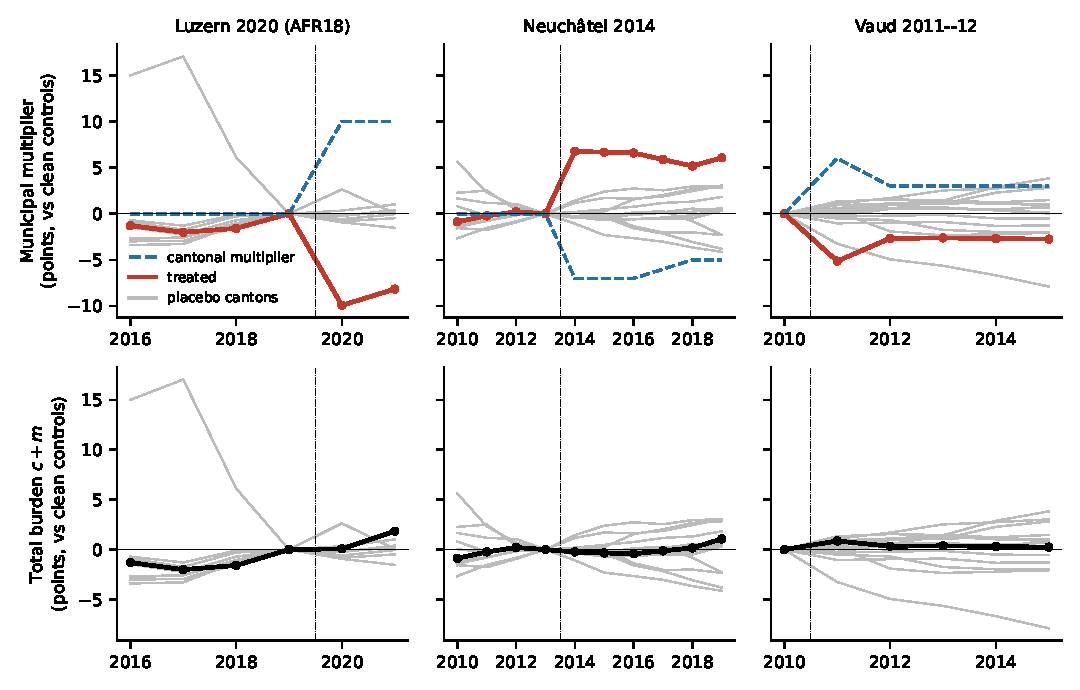
\includegraphics[width=\textwidth]{figs/fig2_swap_es.pdf}
\caption{Mandated swaps: municipal multiplier and combined burden relative to clean control cantons}\label{fig:swapes}
\parbox{0.95\textwidth}{\footnotesize \emph{Notes:} Change since the year before the swap in the average multiplier of stable municipalities in the swapping canton minus the average across control cantons (points). Dashed: the cantonal multiplier. Grey lines: placebo paths, each control canton treated as the swapping canton. The horizon of Luzern ends in 2021 because the canton cut its multiplier by ten points in 2022; Neuch\^atel ends in 2019 and Vaud in 2015. Control cantons: LU: AI, BL, GE, JU, NW, SO, UR, VS; NE: BE, BL, FR, GE, GR, JU, TG, TI, UR, VS, ZG, ZH; VD: AG, BE, BL, BS, FR, GE, GR, JU, TG, TI, UR, VS, ZG, ZH.}
\end{figure}

\begin{table}[t]\centering\small
\begin{threeparttable}
\caption{Municipal multiplier and combined burden after mandated swaps (points, relative to clean controls)}\label{tab:swapes}
\begin{tabular}{llrrrrrr}
\toprule
Event & Outcome & $h=0$ & $h=1$ & $h=2$ & $h=3$ & $h=4$ & $h=5$ \\
\midrule
LU 2020 & Municipal $m$ & $-9.92$ & $-8.16$ & --- & --- & --- & --- \\
        & Combined $c+m$ & $0.08$ & $1.84$ & --- & --- & --- & --- \\
NE 2014 & Municipal $m$ & $6.76$ & $6.67$ & $6.58$ & $5.87$ & $5.17$ & $6.07$ \\
        & Combined $c+m$ & $-0.24$ & $-0.33$ & $-0.42$ & $-0.13$ & $0.17$ & $1.07$ \\
VD 2011 & Municipal $m$ & $-5.13$ & $-2.67$ & $-2.62$ & $-2.69$ & $-2.75$ & --- \\
        & Combined $c+m$ & $0.87$ & $0.33$ & $0.38$ & $0.31$ & $0.25$ & --- \\
\bottomrule
\end{tabular}

\begin{tablenotes}\footnotesize
\item \emph{Notes:} $h$ is the year relative to the swap (VD: 2011). Pre-period gaps for $h=-4,-3,-2$: LU $-1.29,-2.01,-1.59$; NE $-0.87,-0.23,+0.21$ (VD: not available, the sample starts in 2010).
\end{tablenotes}
\end{threeparttable}
\end{table}

\FloatBarrier

Two points deserve emphasis. First, the swaps are highly persistent: the municipal component does not return to its previous level, and in Neuch\^atel and Vaud, with follow-up of four to five years, the combined burden is essentially unchanged. In Luzern the combined burden is $+1.8$ points above controls in 2021, indicating that municipalities reversed on average about 18 percent of the swap after the mandate lapsed (Section~\ref{sec:lu}). Second, the pre-period gaps in Luzern ($-1.3$ to $-2.0$ points) show that Luzern's municipal multipliers rose modestly relative to controls in 2019, before the swap; this cannot explain a gap of $-9.9$ points but shows that base-year noise is of the order of one to two points.

The regression estimate of the same-year offset in equation~\eqref{eq:dl} is $\delta_0=-0.864$ (s.e.\ 0.024), so the pass-through of a swap to the combined burden in the year of the swap is $0.136$. The coefficient at lag 1 is $+0.139$ (0.020) and at lag 2 is $-0.015$ (0.038), a partial reversal in the year after (in Vaud it is the second, mandated step).

\subsection{Unilateral cantonal changes are not offset}

Figure~\ref{fig:dl}(a) and Table~\ref{tab:robust} report the distributed-lag estimates for the 39 unilateral changes. The coefficients are small and of alternating sign: 0.059 (s.e.\ 0.046) contemporaneously, 0.101 (0.023) at lag 1, $-0.158$ (0.022) at lag 2 and $-0.011$ (0.027) at lag 3. Their sum, the cumulative offset, is $-0.008$ (s.e.\ 0.033), with a 95\% confidence interval $[-0.073,\,0.057]$; the permutation $p$-value is 0.81. Pass-through to the combined burden is $0.992$ (s.e.\ 0.033): unilateral cantonal changes reach households in full. The estimate is stable across specifications (Table~\ref{tab:robust}): it lies between $-0.09$ and $+0.10$ in all of them, and $+0.004$ (0.025) when I remove all cantons that have swaps or partial swaps, so that the unilateral class is composed only of cantons in which no municipal offset ever occurs.

The leads are the main threat. The coefficients on leads are positive and precisely estimated ($+0.033$ at $t{+}1$, permutation $p=0.056$; $+0.078$ at $t{+}2$, $p=0.013$): municipal multipliers tend to move in the same direction as the cantonal multiplier before the canton changes it. Two readings are possible. Municipalities and cantons may react to common fiscal conditions, with the cantonal reaction lagging (cantonal budget and referendum cycles are slower); or cantons may partly follow municipalities. Either way, the lags cannot be read as causal responses of municipalities to cantons. Without leads, the cumulative coefficient is $+0.095$ (0.051); allowing canton-specific drift in multipliers, it is $+0.062$ (0.027). If anything, then, municipal and cantonal multipliers \emph{co-move}, which is the opposite of offsetting. In no specification do I find a negative cumulative offset that is distinguishable from zero.

I also examined whether the response differs between hikes and cuts. Without drift controls, municipal multipliers fall by $0.30$ per absolute point (s.e.\ 0.04) after cantonal changes of either sign, which might be read as an asymmetric response. This pattern disappears once canton-specific drift is allowed for ($-0.01$, s.e.\ 0.12; hikes $+0.07$, cuts $+0.15$, neither significant), which indicates that it reflects downward drift in cantons that adjust their multipliers frequently rather than a response to cantonal changes. I therefore do not interpret it.

\begin{figure}[t]\centering
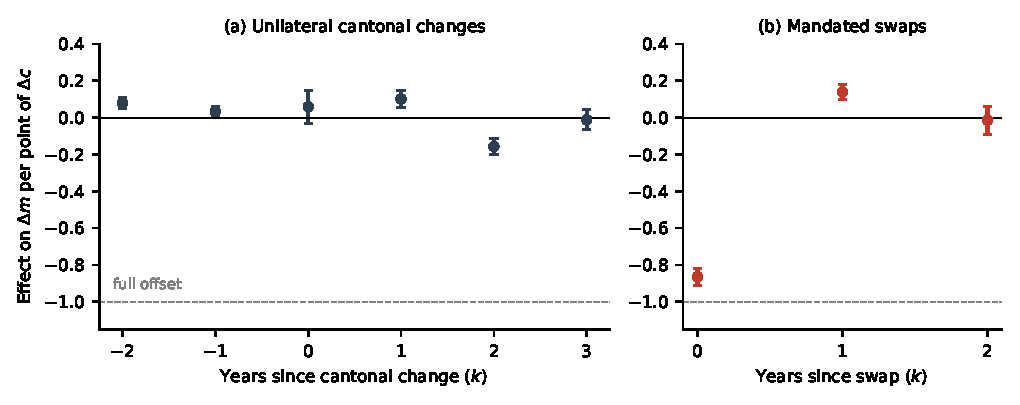
\includegraphics[width=0.92\textwidth]{figs/fig3_dl.pdf}
\caption{Municipal response to cantonal changes: distributed lags}\label{fig:dl}
\parbox{0.95\textwidth}{\footnotesize \emph{Notes:} Coefficients and 95\% confidence intervals (clustered by canton) from equation~\eqref{eq:dl}: effect on the municipal multiplier of one point of cantonal change, by years since the cantonal change. Negative leads/lags are $k<0$. Dashed line: full offset. Panel (b) shows the coefficients on the swap variable.}
\end{figure}

\begin{table}[t]\centering\small
\caption{Cumulative municipal offset of unilateral cantonal multiplier changes: robustness}\label{tab:robust}
\resizebox{\textwidth}{!}{\begin{tabular}{lcccccc}
\toprule
Specification & Cum. offset (0--3) & S.E. & $p$ (cluster) & Lead $t{+}2$ & $N$ & Cantons \\
\midrule
Baseline (3 lags, 2 leads) & -0.008 & (0.033) & 0.81 & 0.078*** & 18,958 & 24 \\
2 lags & -0.019 & (0.039) & 0.64 & 0.125*** & 20,853 & 24 \\
4 lags & -0.065 & (0.089) & 0.47 & 0.087*** & 17,062 & 24 \\
No leads & 0.095 & (0.051) & 0.08 &  & 22,747 & 24 \\
Drop SZ & -0.089 & (0.061) & 0.16 & 0.096*** & 18,658 & 23 \\
Drop SZ, SH & -0.054 & (0.076) & 0.49 & 0.117*** & 18,408 & 22 \\
Drop cantons with swaps/partial swaps & 0.004 & (0.025) & 0.87 & 0.073*** & 13,110 & 15 \\
Include AR & -0.022 & (0.041) & 0.59 & 0.084*** & 19,157 & 25 \\
Trim $|\Delta m|\le 20$ & 0.001 & (0.029) & 0.96 & 0.077*** & 18,916 & 24 \\
\bottomrule
\end{tabular}}

\vspace{2pt}\parbox{\textwidth}{\footnotesize \emph{Notes:} Dependent variable: $\Delta m_{it}$ in points. ``Cum.\ offset'' is $\sum_{\ell=0}^{L}\beta_\ell$ from equation~\eqref{eq:dl}; $-1$ is a full offset, 0 none. All specifications include year fixed effects and the swap variables. Standard errors clustered by canton. ``Lead $t{+}2$'' is the coefficient on the cantonal change two years ahead. $^{*}p<0.10$, $^{**}p<0.05$, $^{***}p<0.01$.}
\end{table}

\subsection{Municipalities do not respond to their neighbours across the cantonal border}

Table~\ref{tab:spatial} reports estimates of equation~\eqref{eq:sp}. The cumulative response of a municipality's multiplier to neighbouring cantonal changes is $-0.049$ (s.e.\ 0.036) in the full sample, $-0.044$ (0.034) when restricted to border municipalities, and $-0.046$ (0.035) with municipality fixed effects. The sign matches strategic substitutability, as found by \citet{Parchet2019} for municipal rates, but the magnitude is small and not distinguishable from zero: the 95\% interval for the full sample is $[-0.12,\,+0.02]$ per point of cantonal change. The coefficient on the lead of the neighbour's change is $0.002$ (0.012), so there is no sign of pre-trends in this design, unlike in the vertical design. The cumulative response to neighbours' \emph{swaps}, that is, to a mandated change in the neighbour's municipal rate that leaves its residents' burden unchanged, is $-0.012$ (0.170); this estimate is too imprecise to rule out mimicry coefficients of the order of $\pm0.3$, so it cannot settle whether headline rates matter. The exposure comprises 47 municipalities adjacent to Luzern, 62 to Vaud and 21 to Neuch\^atel (all municipalities, including those excluded from the stable sample).

\begin{table}[t]\centering\small
\begin{threeparttable}
\caption{Municipal response to neighbouring cantons' multiplier changes}\label{tab:spatial}
\begin{tabular}{lccc}
\toprule
 & (1) All & (2) Border only & (3) + Muni FE \\
\midrule
Neighbour cantonal change, lead $t{+}1$ & 0.002 & 0.013 & 0.005 \\
 & (0.012) & (0.022) & (0.013) \\
Neighbour cantonal change, cum. $t$ to $t{-}2$ & -0.049 & -0.044 & -0.046 \\
 & (0.036) & (0.034) & (0.035) \\
Neighbour mandated swap ($-\Delta c$), lead $t{+}1$ & 0.025 & 0.032 & -0.017 \\
 & (0.066) & (0.074) & (0.066) \\
Neighbour mandated swap, cum. $t$ to $t{-}2$ & -0.012 & -0.115 & -0.108 \\
 & (0.170) & (0.145) & (0.145) \\
\midrule
Canton$\times$year FE & Yes & Yes & Yes \\
Municipality FE & No & No & Yes \\
Observations & 18,958 & 6,558 & 18,958 \\
\bottomrule
\end{tabular}
\begin{tablenotes}\footnotesize
\item \emph{Notes:} Dependent variable: $\Delta m_{jt}$. Regressors follow equation~\eqref{eq:sp}: the average change in the neighbouring cantons' multiplier across cross-border adjacent municipalities, and the average mandated municipal-rate change from neighbouring swaps ($-\Delta c^S$); ``cum.'' is the sum of coefficients at $t$, $t-1$, $t-2$. Standard errors clustered by own canton. $^{*}p<0.10$, $^{**}p<0.05$, $^{***}p<0.01$.
\end{tablenotes}
\end{threeparttable}
\end{table}

\subsection{Luzern: fiscal incidence of the swap and the expiry of the mandate}\label{sec:lu}

\paragraph{Incidence.} Figure~\ref{fig:lu} and Table~\ref{tab:lu} show, for 21 Luzern municipalities with at least 5,000 inhabitants relative to 117 municipalities in control cantons, the evolution of the municipal multiplier and of key financial aggregates. The log gap in the municipal multiplier is $-0.055$ in 2020 and $-0.045$ in 2021, i.e.\ about ten points on an average multiplier of about 1.8 to 2.0. Revenue from direct taxes on natural persons (account 400) falls with a lag: $-0.017$ in 2020, $-0.058$ in 2021 (95\% interval $[-0.086,-0.029]$), $-0.050$ in 2022 and $-0.076$ in 2023, in line with the mechanical prediction of about $-0.055$. The pre-period is not perfectly flat: the 2017 gap in revenue from direct taxes on natural persons is $-0.047$, which I take as an indication of year-to-year noise of about five percent in such comparisons. Transfer revenue (accounts 46x) increases by 28 percent in 2020 and 27 percent in 2021 (interval $[0.185,\,0.360]$) and by 14 percent in 2023, transfer expenditure by 7--11 percent, operating expenditure by 5--9 percent and operating revenue by 3--8 percent. In descriptive terms, the loss of tax revenue is more than compensated by transfers, with both sides of the ledger expanding; the net operating balance, revenue minus expenditure in logs, changes by less than three percentage points in any year, consistent with the design objective of overall neutrality \citep{KantonLU2019}.

\begin{figure}[t]\centering
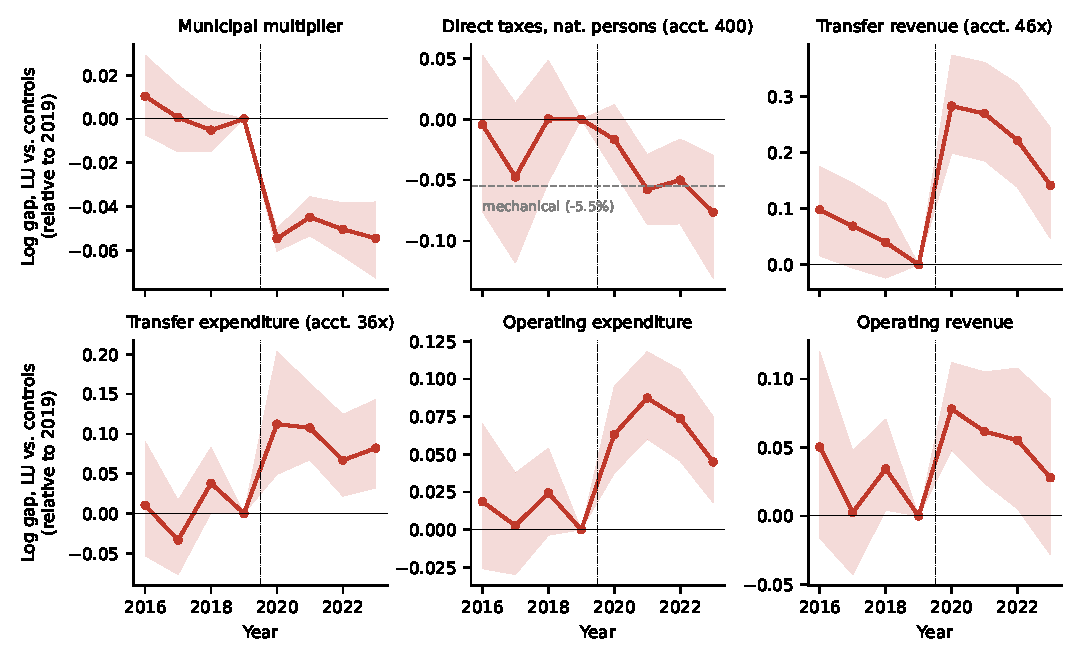
\includegraphics[width=\textwidth]{figs/fig4_lu.pdf}
\caption{Luzern's AFR18: municipal multiplier, taxes, transfers and expenditure relative to control cantons}\label{fig:lu}
\parbox{0.95\textwidth}{\footnotesize \emph{Notes:} Log gap between 21 Luzern municipalities with at least 5,000 inhabitants and 117 municipalities in BL, GE, JU, UR, VS, ZH, relative to 2019. Shaded: 95\% bootstrap interval from resampling municipalities. Dashed line in the tax panel: mechanical prediction from the multiplier cut (about $-5.5$ percent). Account groups follow the FFA classification.}
\end{figure}

\begin{table}[t]\centering\small
\begin{threeparttable}
\caption{Luzern's AFR18: log gap relative to control cantons and 2019}\label{tab:lu}
\begin{tabular}{lcccc}
\toprule
Outcome (log gap vs.\ 2019) & 2020 & 2021 & 2022 & 2023 \\
\midrule
Municipal multiplier & -0.055 & -0.045 & -0.050 & -0.055 \\
Direct taxes, nat. persons (acct. 400) & -0.017 & -0.058 & -0.050 & -0.076 \\
Transfer revenue (acct. 46x) & +0.282 & +0.269 & +0.221 & +0.141 \\
Transfer expenditure (acct. 36x) & +0.112 & +0.107 & +0.067 & +0.082 \\
Operating expenditure & +0.063 & +0.087 & +0.074 & +0.045 \\
Operating revenue & +0.078 & +0.062 & +0.055 & +0.028 \\
\midrule
Municipalities (LU / controls) & \multicolumn{4}{c}{21 / 117} \\
\bottomrule
\end{tabular}
\begin{tablenotes}\footnotesize
\item \emph{Notes:} Point estimates only; only one canton is treated and the comparison is descriptive (Section~\ref{sec:strategy}). The full table with 95\% bootstrap intervals is Appendix Table~\ref{tab:lu_full}.
\end{tablenotes}
\end{threeparttable}
\end{table}

\paragraph{The swap outlived the mandate.} The mandate applied to fiscal year 2020 only and was declared unconstitutional in May 2020 (Section~\ref{sec:inst}). Of the 71 stable Luzern municipalities, only one (1.4 percent) set a multiplier other than the mandated one in 2020, even though municipalities were free to do so after the ruling. In 2021, the first year of completely free choice, 74.6 percent left their multiplier unchanged, 18.3 percent raised it (eleven by ten points, i.e.\ reversing the swap entirely, one by six and one by five) and 7.0 percent lowered it. The mean change is $+1.3$ points, or 13 percent of the swap; relative to controls, the average reversal is 1.8 points (Table~\ref{tab:swapes}). Reversals are lumpy, either full or none. The single deviator in 2020 is Vitznau, which kept its 2019 multiplier of 140 percent. Together with the City of Luzern and the municipality of Meggen, Vitznau was one of the parties that had brought the case to the Federal Supreme Court \citep{BGer2020}; the other two, however, complied with the mandate in 2020. The City of Luzern applied the mandated cut (185 to 175 percent) and left its multiplier unchanged in 2021 as well, while Meggen cut from 99 to 89 percent in 2020 and raised it to 95 percent in 2021, a partial reversal.

\paragraph{Who reversed?} If reversals reflected fiscal need, they should be larger where the reform's projected burden is larger. The Globalbilanz provides a policy-defined measure of that burden. Neither the projected net burden per inhabitant nor the mechanical loss from the swap alone predicts the change in the multiplier in 2021 (Figure~\ref{fig:exposure}): the slope of $\Delta m_{2021}$ on the net burden, per CHF 100 per inhabitant, is $+0.03$ (heteroskedasticity-robust s.e.\ 0.31; randomisation $p=0.94$ from 5,000 two-sided permutations of the exposure across municipalities; $n=71$), and $-0.50$ (0.98) per CHF 100 of swap loss. Results are similar in the 80 municipalities with data for 2019--2022, for the cumulative changes 2019--2021 and 2019--2022, and when controlling for the 2019 multiplier (all $p>0.2$). Municipalities in the highest quartile of burden did not reverse more often than others: 11 percent raised their multiplier, against 17, 6 and 41 percent in the other quartiles. Fiscal capacity, measured by per-capita federal tax yield, has a marginally negative slope in 2021 ($-0.96$ points per standard deviation, s.e.\ 0.53, $p=0.069$), but this lies within the range of placebo years in Luzern and does not replicate in Vaud or Neuch\^atel (Figure~\ref{fig:rebound}). I conclude that reversal was not driven by the fiscal burden of the reform; it looks like lumpy, idiosyncratic budget decisions around an inert default. Because the projection predates the hardship compensation, the net-burden measure overstates losses for the worst-affected municipalities, but the swap-only measure is not affected by this. Multiplier levels show no pre-2020 relation with either exposure and no post-2020 relation either (exposure-by-year coefficients within $\pm1.3$ points, all $p>0.3$). Event-study regressions of per-capita financial outcomes on the projected burden, by contrast, show significant pre-period slopes for operating expenditure and the operating balance (joint pre-trend $p=0.001$ in both cases) in the 21 municipalities with financial data, so I do not interpret exposure-based estimates of fiscal absorption.

\begin{figure}[t]\centering
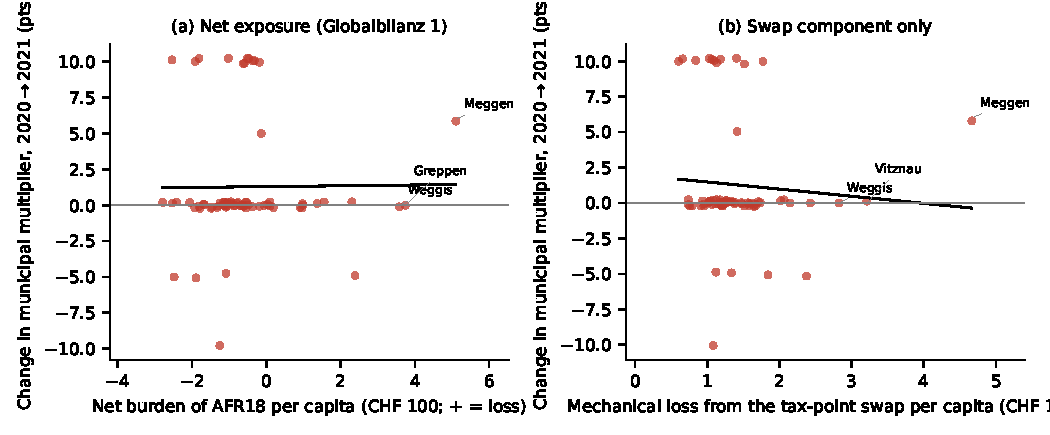
\includegraphics[width=0.95\textwidth]{figs/fig6_exposure.pdf}
\caption{Reversal of the swap and the projected fiscal burden of AFR18}\label{fig:exposure}
\parbox{0.95\textwidth}{\footnotesize \emph{Notes:} Change in the municipal multiplier between 2020 and 2021 against (a) the projected net burden of AFR18 per inhabitant (Globalbilanz 1; CHF 100, positive = burden) and (b) the mechanical revenue loss from the tax-point swap per inhabitant, for 71 stable Luzern municipalities (jittered vertically). Lines: OLS fits.}
\end{figure}

\begin{figure}[t]\centering
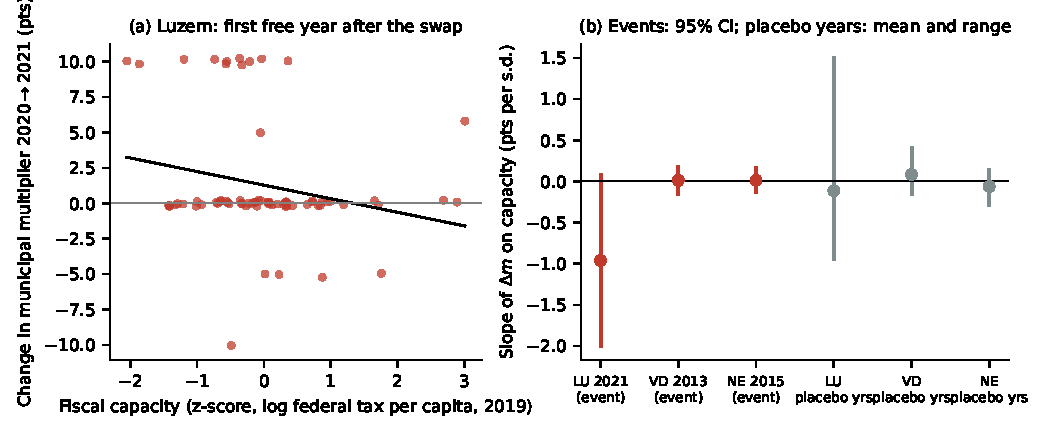
\includegraphics[width=0.95\textwidth]{figs/fig5_rebound.pdf}
\caption{Reversal of the swap and fiscal capacity}\label{fig:rebound}
\parbox{0.95\textwidth}{\footnotesize \emph{Notes:} (a) Change in the municipal multiplier from 2020 to 2021 against fiscal capacity, 71 stable municipalities in Luzern (jittered). (b) Slope of $\Delta m$ on capacity in the first year after the swap episodes (95\% confidence interval) and in years without cantonal changes (mean and range of yearly slopes). Capacity is the z-score of log federal direct tax yield per capita in the last available pre-event year.}
\end{figure}

\subsection{Effective tax burdens}\label{sec:burden}
Multipliers are statutory rates. To check that the main results do not hinge on this choice, I use the effective burden of a single taxpayer without children and without church membership earning CHF 100,000 (Section~\ref{sec:data}), expressed in percentage points of gross income.

\paragraph{Swaps.} Table~\ref{tab:burden_es} repeats the event studies of Section~\ref{sec:swaps} with effective burdens, relative to the year before the swap and to clean control cantons. In Luzern the cantonal burden rises by 0.37 points and the communal burden falls by 0.32 points, so the combined burden changes by 0.05 points (about CHF 50) in 2020 and by 0.15 points in 2021. In Neuch\^atel the changes are $-0.64$ and $+0.66$ points, and the combined burden stays within 0.10 points of its pre-swap level for five years, although it had been falling before the swap (pre-swap gaps of $+0.7$ to $+1.0$ points). In Vaud the combined effective burden rises by 0.13 points in 2011 and by about 0.3 points after four years, more than the multipliers alone suggest; I did not investigate other changes in Vaud's tax law.

\begin{table}[t]\centering\small
\begin{threeparttable}
\caption{Effective burden around mandated swaps (percentage points of gross income)}\label{tab:burden_es}
\begin{tabular}{llrrrrrr}
\toprule
Event & Burden component & $h=0$ & $h=1$ & $h=2$ & $h=3$ & $h=4$ & $h=5$ \\
\midrule
LU 2020 & Cantonal & 0.37 & 0.39 & --- & --- & --- & --- \\
LU 2020 & Communal & -0.32 & -0.24 & --- & --- & --- & --- \\
LU 2020 & Cantonal+communal & 0.05 & 0.15 & --- & --- & --- & --- \\
NE 2014 & Cantonal & -0.64 & -0.64 & -0.65 & -0.63 & -0.52 & -0.50 \\
NE 2014 & Communal & 0.66 & 0.66 & 0.64 & 0.53 & 0.46 & 0.54 \\
NE 2014 & Cantonal+communal & 0.02 & 0.02 & -0.00 & -0.10 & -0.06 & 0.04 \\
VD 2011 & Cantonal & 0.46 & 0.31 & 0.34 & 0.37 & 0.38 & --- \\
VD 2011 & Communal & -0.33 & -0.10 & -0.08 & -0.05 & -0.04 & --- \\
VD 2011 & Cantonal+communal & 0.13 & 0.21 & 0.26 & 0.32 & 0.34 & --- \\
\bottomrule
\end{tabular}
\begin{tablenotes}\footnotesize
\item \emph{Notes:} Single taxpayer, CHF 100,000, no church tax. Change since the year before the swap in the average burden of stable municipalities in the swapping canton, minus the average across clean control cantons (as in Figure~\ref{fig:swapes}); $h$ is the year relative to the swap. Luzern's horizon ends in 2021, Neuch\^atel's in 2019 and Vaud's in 2015.
\end{tablenotes}
\end{threeparttable}
\end{table}

\paragraph{Unilateral changes.} A naive distributed-lag regression of the change in communal burden on the change in cantonal burden gives a positive cumulative coefficient ($+0.14$, s.e.\ 0.07; Table~\ref{tab:burden_dl}). This is mechanical. In 90 of the 390 canton-years since 2011 the cantonal tax schedule or deductions change, which moves the simple tax and therefore both burdens; in 79 of them the multiplier does not change, and in these canton-years the communal burden moves by 0.40 points (s.e.\ 0.19) per point of change in the cantonal burden. I therefore define the cantonal shock as the multiplier-driven change in the cantonal burden, holding the schedule at its previous-year value. The cumulative offset is then $-0.10$ (s.e.\ 0.07; 95\% interval $[-0.23,\,0.03]$), the swap coefficient is $-0.87$ (0.09), and excluding Valais and Geneva changes nothing. The conclusion of no detectable voluntary offset survives, but the effective-burden estimate is less precise and cannot exclude offsets of up to about a quarter of the cantonal change.

\begin{table}[t]\centering\small
\caption{Effective-burden check of the voluntary offset}\label{tab:burden_dl}
\resizebox{\textwidth}{!}{\begin{tabular}{lccc}
\toprule
Outcome and cantonal shock & Cum. offset (0--3) & S.E. & Swap, same year \\
\midrule
Multiplier change, multiplier shock (baseline) & $-0.008$ & (0.033) & $-0.864$ (0.024) \\
Communal burden, cantonal burden change (naive) & $+0.144$ & (0.068) & $-0.970$ (0.068) \\
Communal burden, multiplier-driven cantonal shock & $-0.099$ & (0.066) & $-0.874$ (0.089) \\
\bottomrule
\end{tabular}}

\vspace{2pt}\parbox{\textwidth}{\footnotesize \emph{Notes:} Same sample as Table~\ref{tab:robust} (18,958 municipality-years, 24 cantons), year fixed effects, standard errors clustered by canton. The multiplier-driven shock is the change in the cantonal multiplier times the cantonal simple tax of the previous year.}
\end{table}

\section{Discussion and limitations}\label{sec:disc}

\paragraph{Interpretation.} I find no evidence that municipalities internalise the vertical externality on their own. In the swap episodes I identify, the combined statutory burden is held approximately constant by the design of the reform (documented for Luzern). Across the 45 events, cantons change their multipliers without a simultaneous municipal counter-move in the large majority of cases (39 of 45), and municipalities do not exhibit a detectable offset in the following years; the combined statutory burden moves almost one-for-one with the cantonal change (pass-through 0.99). The persistence of the swaps points in the same direction: reallocation of tax points between tiers is not undone by municipalities, even when the mandate ceases to bind. This is consistent with substantial inertia in local rate setting, in which the status quo is the default outcome of the budget process. The Luzern evidence on who reversed points the same way: the projected fiscal burden of the reform does not predict which municipalities reversed the swap once they were free to do so. The inertia reading is not the only one available, though. It may instead reflect that swaps were compensated through offsetting task or transfer changes, so that municipalities had no fiscal reason to reverse them regardless of how strong their attachment to the status quo happened to be; the two accounts are not mutually exclusive, and the data at hand cannot fully separate them.

\paragraph{Limitations.} First, multipliers are statutory rates on the simple tax, not effective burdens; where cantons change tax schedules in the same year as multipliers, the combined multiplier mismeasures the change in burden. Section~\ref{sec:burden} checks the main results with effective burdens for a single taxpayer earning CHF 100,000, but other households and income levels are not covered. Second, the lead coefficients show that municipal and cantonal multipliers are correlated ahead of cantonal changes, so I read the voluntary-response estimates as bounds on offsetting rather than as sharp causal effects; canton-specific drift moves the cumulative coefficient from $-0.01$ to $+0.06$. Third, there are only 24 canton clusters, and only three swapping cantons with sufficient municipalities. Fourth, the stable sample excludes municipalities involved in mergers, roughly a quarter of all identifiers, and the results need not extend to them. Fifth, the analysis weights municipalities equally; the financial statistics cover only municipalities with at least 5,000 inhabitants, and for Luzern the case study measures average, not net-of-compensation, exposure because the aggregate balance (\emph{Gesamtbilanz}) per municipality is not used. Sixth, the Luzern exposure is a projection from the ballot brochure that predates the hardship compensation. Seventh, cross-border exposure is based on current polygons for adjacency. Finally, I do not test the hypothesis of headline-rate competition with sufficient power.

\section{Conclusion}\label{sec:concl}

In the data, near-complete offsetting between cantonal and municipal multipliers occurs in a few episodes consistent with mandated swaps. Four large swaps offset almost one-for-one, leave the combined statutory burden approximately unchanged and, in two cases, persist for years, while for 39 other cantonal changes I find no detectable municipal offset and no precisely estimated cross-border response. Luzern's AFR18 shows that a swap can come with large gross reallocations of transfers and expenditure, and that a mandated reallocation can become the default that municipalities keep even when the legal requirement lapses.

Three extensions would strengthen the analysis. First, replacing multipliers with effective burdens (from the ESTV burden statistics) would remove the schedule-change concern. Second, using each Luzern municipality's aggregate net balance under AFR18 as a continuous exposure would allow a within-canton test of how fiscal windfalls and losses are absorbed. Third, the design carries over to corporate taxation: the 2020 federal tax reform (STAF) prompted cantons to cut profit-tax rates and compensate municipalities, which is a setting in which vertical and horizontal interaction over a mobile base can be studied with the same data.

\bigskip\noindent\textbf{Data and code.} All analysis scripts accompany this draft. The data are public: ESTV multipliers, ESTV federal-direct-tax statistics, and ESTV effective tax-burden statistics (Swiss Tax Calculator); FFA municipal financial statistics; the BFS historised municipality register (eCH-0071, 1 January 2026); swisstopo swissBOUNDARIES3D (2026); and Kanton Luzern's Globalbilanz 1 for the AFR18 reform.

\renewcommand{\bibfont}{\small}
\bibliographystyle{plainnat}
\bibliography{references}

\appendix
\section{Data construction}\label{app:data}
\paragraph{Merger identification.} The historised municipality register lists every municipality record with an admission and, where applicable, an abolition mutation number. A mutation with abolition mode 29 (dissolution) and an effective year between 2011 and 2025 (the day after the abolition date) is a merger; a municipality identifier is merger-involved if any of its records is abolished or admitted in such a mutation. This yields 754 identifiers, of which 562 no longer exist in the 2026 boundaries. Of the 570 codes that disappear from the multiplier panel, 97.5 percent are in this set.

\paragraph{Stable sample.} A municipality is stable if it appears in every year of the multiplier panel, is in the 2026 boundaries and is not merger-involved. In the 16 annual ESTV files, 2,026 codes appear in every year; 103 of them are merger-involved (mostly absorbing municipalities that keep their code) and seven are absent from the 2026 boundaries, which leaves 1,916 municipalities. Estimation samples further exclude Appenzell Ausserrhoden, observations with $|\Delta m|>40$ points (nine municipality-years, in AR, BE, NW, OW and SZ) and years without the required leads and lags; the baseline sample of equation~\eqref{eq:dl} has 18,958 municipality-years, 1,896 municipalities and 24 cantons (Glarus has no stable municipality).

\paragraph{Adjacency.} Polygons of the 2026 boundaries are dissolved by municipality number, and two municipalities are adjacent if their polygons intersect; cross-canton pairs are those with different canton numbers.

\section{Canton-level events}
{\small\setlength{\tabcolsep}{3.3pt}
\begin{longtable}{llrrrrrrl}
\caption{Canton-level multiplier changes of at least 2 points, 2011--2025, and same-year municipal response}\label{tab:events}\\
\toprule
Canton & Year & $c_{t-1}$ & $\Delta c$ & $N$ & Mean $\Delta m$ & Share offset & Share unchanged & Class \\
\midrule
\endfirsthead
\toprule
Canton & Year & $c_{t-1}$ & $\Delta c$ & $N$ & Mean $\Delta m$ & Share offset & Share unchanged & Class \\
\midrule
\endhead
AG & 2018 & 109 & +3.0 & 183 & -1.44 & 0.55 & 0.30 & Unilateral \\
AI & 2011 & 85 & +11.0 & 4 & -10.00 & 0.25 & 0.00 & Small-canton swap \\
BE & 2021 & 306 & -3.5 & 302 & +0.16 & 0.00 & 0.94 & Unilateral \\
BE & 2025 & 302 & -5.0 & 302 & +0.47 & 0.02 & 0.86 & Unilateral \\
BS & 2017 & 55 & -5.0 & 3 & +4.33 & 0.67 & 0.00 & Small-canton swap \\
FR & 2021 & 100 & -2.0 & 98 & +0.40 & 0.01 & 0.88 & Unilateral \\
FR & 2022 & 98 & -2.0 & 98 & +0.01 & 0.00 & 0.92 & Unilateral \\
GR & 2024 & 100 & -5.0 & 75 & -1.17 & 0.00 & 0.84 & Unilateral \\
LU & 2014 & 150 & +10.0 & 71 & +2.31 & 0.04 & 0.76 & Unilateral \\
LU & 2020 & 160 & +10.0 & 71 & -9.86 & 0.99 & 0.01 & Mandated swap \\
LU & 2022 & 170 & -10.0 & 71 & -1.34 & 0.01 & 0.77 & Unilateral \\
LU & 2025 & 160 & -5.0 & 71 & -0.28 & 0.00 & 0.82 & Unilateral \\
NE & 2014 & 130 & -7.0 & 17 & +7.00 & 1.00 & 0.00 & Mandated swap \\
NW & 2013 & 263 & +3.0 & 11 & -7.09 & 0.45 & 0.27 & Unilateral \\
OW & 2015 & 295 & +10.0 & 7 & +9.29 & 0.00 & 0.71 & Unilateral \\
OW & 2020 & 305 & +30.0 & 7 & -12.71 & 0.43 & 0.43 & Unilateral \\
OW & 2025 & 335 & -10.0 & 7 & +4.29 & 0.14 & 0.71 & Unilateral \\
SG & 2012 & 95 & +10.0 & 68 & -1.76 & 0.03 & 0.63 & Unilateral \\
SG & 2013 & 105 & +10.0 & 68 & +0.09 & 0.00 & 0.75 & Unilateral \\
SG & 2022 & 115 & -5.0 & 68 & -2.31 & 0.00 & 0.50 & Unilateral \\
SG & 2023 & 110 & -5.0 & 68 & -1.93 & 0.00 & 0.56 & Unilateral \\
SH & 2016 & 112 & +3.0 & 25 & -0.48 & 0.24 & 0.68 & Unilateral \\
SH & 2018 & 115 & -4.0 & 25 & -0.24 & 0.04 & 0.76 & Unilateral \\
SH & 2020 & 110 & -5.0 & 25 & +0.12 & 0.04 & 0.76 & Unilateral \\
SH & 2021 & 105 & -3.0 & 25 & -0.08 & 0.00 & 0.96 & Unilateral \\
SH & 2022 & 102 & -10.0 & 25 & -0.12 & 0.00 & 0.96 & Unilateral \\
SH & 2023 & 92 & -3.0 & 25 & -0.36 & 0.00 & 0.80 & Unilateral \\
SH & 2024 & 89 & -8.0 & 25 & -0.56 & 0.00 & 0.68 & Unilateral \\
SH & 2025 & 81 & -2.0 & 25 & -0.48 & 0.00 & 0.76 & Unilateral \\
SO & 2012 & 104 & -4.0 & 97 & +0.55 & 0.08 & 0.79 & Unilateral \\
SO & 2014 & 100 & +2.0 & 97 & +0.31 & 0.00 & 0.85 & Unilateral \\
SO & 2015 & 102 & +2.0 & 97 & +0.80 & 0.01 & 0.81 & Unilateral \\
SZ & 2015 & 120 & +25.0 & 30 & +4.20 & 0.00 & 0.47 & Unilateral \\
SZ & 2016 & 145 & +25.0 & 30 & -0.57 & 0.00 & 0.60 & Unilateral \\
SZ & 2019 & 170 & -10.0 & 30 & -2.10 & 0.00 & 0.47 & Unilateral \\
SZ & 2020 & 160 & -10.0 & 30 & -4.17 & 0.00 & 0.37 & Unilateral \\
SZ & 2022 & 150 & -30.0 & 30 & -5.13 & 0.00 & 0.37 & Unilateral \\
SZ & 2025 & 120 & -5.0 & 30 & -14.70 & 0.00 & 0.03 & Unilateral \\
TG & 2022 & 117 & -8.0 & 80 & -2.27 & 0.00 & 0.39 & Unilateral \\
TI & 2020 & 100 & -3.0 & 83 & -0.17 & 0.01 & 0.87 & Unilateral \\
TI & 2024 & 97 & +3.0 & 83 & -0.16 & 0.04 & 0.88 & Unilateral \\
VD & 2011 & 152 & +6.0 & 278 & -5.76 & 0.87 & 0.01 & Mandated swap \\
VD & 2012 & 158 & -3.0 & 278 & +2.09 & 0.83 & 0.08 & Mandated swap \\
ZG & 2021 & 82 & -2.0 & 11 & +0.19 & 0.09 & 0.91 & Unilateral \\
ZG & 2024 & 80 & +2.0 & 11 & -1.62 & 0.55 & 0.27 & Unilateral \\
\bottomrule
\multicolumn{9}{p{0.95\textwidth}}{\footnotesize \emph{Notes:} $c_{t-1}$: cantonal income-tax multiplier in the previous year (\% of the simple tax). $N$: number of stable municipalities in the canton. ``Share offset'': share of municipalities with $|\Delta m+\Delta c|\le 1$. ``Share unchanged'': share with $\Delta m=0$. Appenzell Ausserrhoden (2014, 2018) is excluded because of implausible municipal jumps in the source data.}\\
\end{longtable}
}

\section{Luzern's AFR18: full results}
Table~\ref{tab:lu_full} reproduces Table~\ref{tab:lu} with 95\% bootstrap confidence intervals (in brackets, from resampling municipalities), rotated to landscape orientation for legibility.

\begin{landscape}
\begin{table}[t]\centering\small
\begin{threeparttable}
\caption{Luzern's AFR18: log gap relative to control cantons and 2019, with 95\% confidence intervals}\label{tab:lu_full}
\begin{tabular}{lcccc}
\toprule
Outcome (log gap vs.\ 2019) & 2020 & 2021 & 2022 & 2023 \\
\midrule
Municipal multiplier & -0.055 & -0.045 & -0.050 & -0.055 \\
 & [-0.060, -0.050] & [-0.053, -0.036] & [-0.063, -0.038] & [-0.073, -0.038] \\
Direct taxes, nat. persons (acct. 400) & -0.017 & -0.058 & -0.050 & -0.076 \\
 & [-0.043, +0.012] & [-0.086, -0.029] & [-0.086, -0.016] & [-0.131, -0.030] \\
Transfer revenue (acct. 46x) & +0.282 & +0.269 & +0.221 & +0.141 \\
 & [+0.198, +0.373] & [+0.185, +0.360] & [+0.138, +0.322] & [+0.046, +0.244] \\
Transfer expenditure (acct. 36x) & +0.112 & +0.107 & +0.067 & +0.082 \\
 & [+0.049, +0.203] & [+0.067, +0.164] & [+0.022, +0.124] & [+0.032, +0.143] \\
Operating expenditure & +0.063 & +0.087 & +0.074 & +0.045 \\
 & [+0.038, +0.095] & [+0.060, +0.118] & [+0.046, +0.106] & [+0.018, +0.075] \\
Operating revenue & +0.078 & +0.062 & +0.055 & +0.028 \\
 & [+0.048, +0.112] & [+0.024, +0.105] & [+0.005, +0.108] & [-0.028, +0.085] \\
\midrule
Municipalities (LU / controls) & \multicolumn{4}{c}{21 / 117} \\
\bottomrule
\end{tabular}
\begin{tablenotes}\footnotesize
\item \emph{Notes:} 95\% bootstrap intervals in brackets, from resampling the 21 Luzern and 117 control municipalities. Only one canton is treated; the comparison is descriptive (Section~\ref{sec:strategy}). This table reports the same estimates as Table~\ref{tab:lu} in the main text.
\end{tablenotes}
\end{threeparttable}
\end{table}
\end{landscape}

\end{document}
